\documentclass[11pt,a4paper]{article}
\usepackage[margin=2.4cm]{geometry}
\usepackage[T1]{fontenc}
\usepackage{lmodern}
\usepackage{microtype}
\usepackage{booktabs}
\usepackage{longtable}
\usepackage{array}
\usepackage{enumitem}
\usepackage{xcolor}
\usepackage{tikz}
\usetikzlibrary{positioning,arrows.meta,fit}
\usepackage[colorlinks=true,linkcolor=blue!50!black,urlcolor=blue!50!black,citecolor=blue!50!black]{hyperref}
\usepackage{url}

\newcommand{\todo}[1]{\textcolor{red!70!black}{[#1]}}
\newcommand{\est}{\textsuperscript{est}}

\title{An open focused- and functional-ultrasound bench for brain research:\\
what to build on, what to buy, and what to build}
\author{Morgan Hough (m9h)\thanks{Draft prepared with Claude Code; facts were checked against the sources listed in the bibliography on 2026-10-25 unless marked \todo{check}. Prices marked \est{} are rough estimates to be confirmed with vendors.}\\
\small for neurotech@berkeley, with Jean Rintoul as advisor}
\date{Draft 0.2 --- 25 October 2026}

\begin{document}
\maketitle

\begin{abstract}
Ultrasound has become the most active non-invasive route into the brain: functional ultrasound (fUS) imaging gives fMRI-like maps at sub-second, sub-100\,\textmu m resolution; transcranial ultrasound stimulation (TUS) now reaches deep structures such as the thalamus in humans with electronically steered arrays; and acoustoelectric methods promise a direct electrical readout focused by sound. Until 2025 the hardware for all three was closed and expensive. That has changed: Openwater released its whole medical-device portfolio as open source, including the Open-LIFU stimulation stack (CERN-OHL-S hardware, Apache/AGPL software) and a patent pledge over its 68 filings; Aleph Neuro published an MIT-licensed 3D transcranial ultrasound-localisation-microscopy pipeline with data in June 2026; and in October 2026 NVIDIA released the Holoscan Ultrasound Imaging Reference Design, an Apache-licensed, roughly \$10k\est{} raw-channel imaging machine that streams 128\,TX/64\,RX channel data straight into GPU memory and names the DGX Spark as its host.
This document lays out a plan for a student-built research bench of the kind Arbor Neuroscience (formerly Forest Neurotech) is building at far larger scale: an imaging-plus-stimulation ultrasound system with simulation-based planning, neuronavigation, calibrated safety limits, and an acoustoelectric readout path. It reviews the recent history (Paris/Iconeus, Oxford/UCL, Nudge, Forest/Arbor and Merge Labs, Butterfly Network and its Embedded partners Aleph Neuro, Bridge Neurotech and Midjourney Medical), surveys the patent landscape that an open project has to navigate, catalogues the open software to build on (Openwater's Open-LIFU and Open-Motion, Aleph's ULM pipeline, the Neurotech Development Kit from AE Studio, BabelBrain/BabelViscoFDTD, k-Wave/j-Wave, PRESTUS, SimNIBS, our own \texttt{ae-sim}), gives a first bill of materials, and names the pieces that do not yet exist and would have to be built. Everything here is for phantom and bench work; no human use is proposed.
\end{abstract}

\tableofcontents

\section{Why now}

Three things happened within eighteen months of each other.

\begin{enumerate}[leftmargin=*]
\item \textbf{Deep TUS in humans with a steerable array.} In September 2025 Martin, Treeby, Stagg and colleagues at UCL and Oxford reported a 256-element, 555\,kHz helmet array with real-time fMRI monitoring that selectively modulated the lateral geniculate nucleus in seven volunteers, suppressing visual-cortex activity for at least 40\,minutes after a theta-burst protocol \cite{martin2025}. This is the first demonstration that electronically focused, individually planned deep-brain TUS works in people.
\item \textbf{Open hardware for both stimulation and imaging.} Openwater's Open-LIFU (2024--2025) published the transducer flex, transmit module and console as CERN-OHL-S designs with an Apache-licensed Python toolbox and a 3D~Slicer extension \cite{openlifu}. In October 2026 NVIDIA, with TI, Terasic and Sonosray, published the Holoscan Ultrasound Imaging Reference Design: an Apache-2.0 host stack plus FPGA IP that streams raw RF from a 128\,TX/64\,RX front end over 100\,GbE into GPU memory and lets the GPU set the next transmit shot at about 1\,500 updates per second \cite{holoscan,simson2026}. The project page names the DGX Spark (GB10) as a host; we already have one.
\item \textbf{Capital and credibility.} Nudge raised \$100M in July 2025 for MRI-guided low-intensity focused ultrasound and is running a 150-participant essential-tremor study \cite{nudge}. Forest Neurotech, a Convergent Research focused research organisation, started an NHS safety study of its wearable fUS imager over craniectomy windows in March 2025 with \pounds6.5M from ARIA \cite{forest1}, was renamed Arbor Neuroscience, and spun out Merge Labs, which emerged in January 2026 with \$252M including OpenAI \cite{merge}. In 2026 Butterfly Network turned its Ultrasound-on-Chip into a licensed platform for brain interfaces (Aleph Neuro in June, Merge Labs in September, Bridge Neurotech in October) and for Midjourney Medical's whole-body scanner \cite{bfly_aleph,bfly_merge,bfly_bridge,bfly_midjourney}.
\end{enumerate}

Students can now assemble, from published designs and open code, a bench that would have been a seven-figure Verasonics-and-custom-array project five years ago. The purpose of this plan is to say exactly which pieces exist, which can be bought, and which still have to be made.

\section{A short recent history}

\subsection{Functional ultrasound imaging: Paris and Iconeus}

Functional ultrasound began in Mickael Tanter's group at ESPCI Paris (now Physics for Medicine Paris, Inserm/CNRS/ESPCI). The 2011 insight was that ultrafast plane-wave imaging, at thousands of frames per second, raises Doppler sensitivity enough to see cerebral blood volume changes in small vessels, and therefore neurovascular coupling, first in rodents \cite{iconeus_story}. With Zsolt Lenkei and Bruno Osmanski the group showed resting-state functional connectivity in rat, then awake and freely moving animals. Iconeus was founded in 2016 by Tanter, Lenkei, Osmanski, Mathieu Pernot, Thomas Deffieux and CEO Ludovic Lecointre to commercialise fUS; Inserm, CNRS and ESPCI licensed the technology in February 2018 \cite{iconeus_story}. The Iconeus One is a portable plane-wave station with a motorised probe platform for head-fixed animals; with ultrasound localisation microscopy (ULM) the same hardware resolves vessels of a few micrometres \cite{iconeus_one}. Iconeus opened a US subsidiary in 2026 \cite{iconeus_us}.

The human-BCI branch of fUS came out of Caltech: Sumner Norman, with the Andersen and Shapiro labs, decoded movement intentions from fUS in non-human primates (2021) and later demonstrated online fUS-BCI control \todo{check exact papers; Norman et al.\ Neuron 2021, Griggs et al.\ Nat.\ Neurosci.\ 2024}. Norman went on to co-found Forest Neurotech and, in 2025, Merge Labs \cite{merge}.

\subsection{Transcranial ultrasound stimulation: Oxford, UCL and the consortium}

Human low-intensity TUS dates to Legon and colleagues (2014) modulating somatosensory cortex \todo{check}. Oxford's contribution was systematic primate work (Fouragnan, Sallet, Rushworth, Verhagen, Folloni, 2019 onward) showing offline effects lasting an hour or more from deep targets such as the amygdala and anterior cingulate \todo{check citations}. UCL's Biomedical Ultrasound Group (Treeby, Cox, Martin) supplied the physics: k-Wave \cite{kwave}, its JAX successor j-Wave \cite{jwave}, skull aberration-correction methods, and the ITRUSST consortium's safety consensus for TUS \cite{itrusst} \todo{add the ITRUSST reporting-standards paper}. The 2025 helmet system \cite{martin2025} is the union of these lines: an individually planned, aberration-corrected, 256-element array with stereotactic positioning and real-time fMRI readout. Elsa Fouragnan's Plymouth group (BRIC) holds the ARIA award with Forest/Arbor for mood-disorder stimulation \cite{forest1}.

\subsection{Nudge}

Nudge (San Francisco, founded 2024 by Fred Ehrsam, Jeremy Barenholtz and Quintin Frerichs) raised a \$100M Series~A in July 2025 led by Thrive Capital and Greenoaks. Its first device, Nudge Zero, is an MRI-guided LIFU system; the first study enrols up to 150 adults with essential tremor for multiple two-to-three-hour in-scanner sessions over three weeks and is explicitly exploratory rather than a safety or efficacy trial. Job postings from March 2026 describe a non-invasive device that both stimulates and images at high resolution and depth \cite{nudge}. Nothing of Nudge's is open.

\subsection{Forest Neurotech, Arbor Neuroscience and Merge Labs}

Forest Neurotech was created as a focused research organisation under Convergent Research to build a ``whole-brain'' ultrasound interface: fUS imaging first, stimulation second, with the transducer eventually small enough to sit in a skull replacement. AE~Studio supported Forest's data science and software \cite{aestudio}. Its first device, Forest~1, is a wearable, miniaturised fUS imager placed on the scalp over a craniectomy window; the UK HRA summary describes a single-centre exploratory study of fUS imaging of brain states via a craniectomy window, running three and a half years from March 2025 \cite{forest1}. Job postings describe Forest~1 as ``a wearable functional MRI, but with higher resolution'' that ``will soon stimulate as well'' \cite{arbor}. The organisation has since been renamed \textbf{Arbor Neuroscience}; it remains a non-profit FRO and describes its programme as measure--intervene--measure in the same individual over months \cite{arbor}.

In December 2025 \emph{Wired} reported that \textbf{Merge Labs} was being spun out of Forest, co-founded by Forest's CEO Sumner Norman and CSO Tyson Aflalo; Forest/Arbor continues independently and collaborates with Merge. Merge emerged in January 2026 with a \$252M seed round including OpenAI, Bain Capital and Gabe Newell, to read from and modulate the brain with non-invasive ultrasound \cite{merge}. (The phrase ``Forest is now part of Merge'' is therefore not quite right: Merge is the for-profit spin-out, Arbor is the continuing non-profit.)

\subsection{Butterfly Network and the chip-based ultrasound BCIs}\label{sec:butterfly}

The other hardware line into the brain is the capacitive micromachined ultrasound transducer on CMOS. Butterfly Network's Ultrasound-on-Chip puts thousands of elements and their electronics on one die; its licensing and co-development business, Butterfly Embedded (formerly Octiv), is now the hardware base for most new ultrasound-BCI companies. Forest Neurotech signed a five-year co-development agreement with Butterfly in October 2023 \cite{bfly_forest}. In 2026 the pace picked up:

\begin{itemize}[leftmargin=*,nosep]
\item \textbf{Aleph Neuro} (Boston; Marley Xiong, Raffi Hotter, Lev Chizhov) launched on 25 June 2026 with what it calls the highest-resolution 3D images of a living human brain taken from outside the skull: ultrasound localisation microscopy of the cerebral vasculature through the intact skull, about four minutes of acquisition under continuous microbubble infusion, on Butterfly chips \cite{bfly_aleph,aleph}. Unusually, Aleph released the whole pipeline and a 96\,GB raw dataset as \texttt{alephneuro/microbubbles} under the MIT licence: MACH GPU beamforming (CUDA 12/13), temporal SVD clutter filtering, 3D sub-voxel bubble localisation, Kalman--Hungarian track linking and browser viewers \cite{aleph_repo}. The result is company-reported and not yet peer reviewed, and it uses contrast; Aleph says it is collecting a large non-contrast neurovascular dataset next. For us this is the first open, GPU-based, raw-channel-to-vascular-map code in the field and it fills part of the fUS gap identified below.
\item \textbf{Merge Labs} signed a multi-year licence on 1 September 2026 for Butterfly's Poseidon family of Ultrasound-on-Chip devices; Butterfly's CEO called Merge its exclusive BCI research-and-development platform partner, and held an invite-only BCI Innovation Summit the next day \cite{bfly_merge}. Merge's stated approach pairs ultrasound with molecular, gene-encoded reporters and actuators from Mikhail Shapiro's Caltech lab rather than electrodes \cite{merge}.
\item \textbf{Bridge Neurotech} (Redwood City; founder Will Biederman, who earlier helped start Forest) came out of stealth on 6--7 October 2026 with \$13.5M and a multi-year Butterfly Embedded agreement (technology-access payments, milestones, hardware purchase commitments) for a fully non-invasive, oxygenated-blood-flow BCI; its first human study is enrolling \cite{bfly_bridge}.
\item \textbf{Midjourney Medical} announced on 17--18 June 2026 a whole-body ``Ultrasonic CT'' scanner: a shallow water bath ringed by Butterfly modules through which a person is lowered, roughly 60\,s per scan as the target (about 20\,min for the Gen-1 prototype), first site in San Francisco planned for late 2027, body-composition maps first because they need no FDA clearance. Butterfly's own release says the prototype uses 40 Ultrasound-on-Chip modules per system, under a co-development deal disclosed in a November 2025 8-K worth up to \$74M over five years \cite{bfly_midjourney}. It is a prototype about a dozen people have been through, and radiologists have been sceptical; but it shows what several hundred thousand CMUT elements and a GPU can do, and the ``ring of chips plus water bath'' is a transmission-tomography geometry, not a transcranial one.
\end{itemize}

None of the Butterfly chips, firmware or SDKs are open, and Embedded is a negotiated licence; a student group cannot buy Poseidon modules. The open route to the same class of data is the Holoscan design (piezo probe, discrete AFE) for raw channels, and Aleph's pipeline for the processing. Gestala (Chengdu), which raised about \$62M in July 2026, is the equivalent Chinese ultrasound-BCI start-up \cite{gestala}.

\subsection{Acoustoelectric readout}

The acoustoelectric effect, the pressure dependence of tissue conductivity, lets a focused ultrasound beam tag the local electric field so that it can be recovered from surface electrodes at the ultrasound frequency. Jean Rintoul (PhD with Nir Grossman at Imperial; founder of Mindseye Labs) showed remote focused encoding and decoding of electric fields through acoustoelectric heterodyning (\emph{Communications Physics}, 2023) and reviewed simple open ultrasound hardware in the \emph{Journal of Open Hardware} (2022) \cite{rintoul}. This is the path by which an imaging-grade array could become an electrical, not only haemodynamic, readout, and it is why our own \texttt{ae-sim} project (Section~\ref{sec:aesim}) matters here.

\subsection{Openwater: the whole portfolio, not only Open-LIFU}\label{sec:openwater}

Openwater (Mary Lou Jepsen) announced in January 2024 that it would open-source everything: hardware blueprints, firmware, software, patents, phantom designs, measurement data and its FDA correspondence \cite{openwater_open}. On 2026-10-25 the \texttt{OpenwaterHealth} GitHub organisation held 56 repositories, every one pushed within the last three weeks \cite{openwater_gh}. They fall into six groups, and more of them are useful to this bench than Open-LIFU alone:

\begin{description}[leftmargin=*,nosep]
\item[Open-LIFU (stimulation).] \texttt{openlifu-electrical} and \texttt{openlifu-mechanical} (CERN-OHL-S-2.0): the 64-element array flex, HV transmit module Rev~0.4.1, console power PCB, housings and tank fixtures, with Gerbers, STEP and BOMs. Firmware (Apache-2.0): \texttt{openlifu-transmitter-fw} (STM32L443), \texttt{openlifu-console-fw}, secure-boot loaders. Software (Apache-2.0): \texttt{openlifu-python} (planning, simulation, transducer control), \texttt{openlifu-sdk} (standalone hardware I/O for the TX module and HV controller), the Qt desktop planner, \texttt{openlifu-test-app}, \texttt{openlifu-verification-tank} (tank control), \texttt{OpenLIFU-3DScanner} and \texttt{OpenLIFU-3DRegistration} (AGPL) for transducer localisation, \texttt{openlifu-closed-loop-eeg}, and \texttt{SlicerOpenLIFU}; \texttt{openlifu-sample-database} (CC~BY~4.0) gives transducer configurations and protocols. Kitware co-develops the software \cite{openlifu}.
\item[Earlier neuromodulation generation.] \texttt{openwater-neuromod-hardware} and \texttt{-software} (AGPL-3.0; the most-starred repositories) hold the wearable, steerable headset and transmit modules described in Bawiec et al.\ 2025 \cite{bawiec2025}, plus acoustic validation files, and \texttt{opw\_ustx} / \texttt{st-ustx*} are the ultrasound transmit module lineage that became the Open-LIFU TX module. These show how the design evolved and contain validation data Open-LIFU does not yet repeat.
\item[Open-Motion (optical blood flow).] A near-infrared optical blood-flow and micro-motion monitor: console with safety, seed and timing FPGAs, camera module FPGA, sensor firmware, \texttt{openmotion-sdk} and a research desktop app (Apache-2.0; FPGA projects AGPL-3.0; PCBs and CAD CERN-OHL-S-2.0) \cite{openwater_gh,openwater_docs}. For a stimulate-then-measure bench it is a second, non-acoustic haemodynamic readout that can run during sonication without interfering with the ultrasound receive chain.
\item[Oncolysis and laser.] \texttt{openwater-oncolysis-*} (preclinical harmonic-excitation data, hardware, software) and \texttt{openwater-laser}; not for this bench, but the oncolysis data is the only open dataset of therapeutic-ultrasound tissue effects we know of.
\item[Shared assets.] \texttt{openwater-phantoms} (AGPL-3.0): recipes and CAD for optical, ultrasound and acousto-optic phantoms, namely a gelatin/agarose recipe sheet and a 67\,MB Gen2 construction-notes PDF for the ultrasound and acousto-optic tissue phantoms, a rat-body mould with vein and artery target moulds (STL, STEP, Rhino), the Gen2/2.5 optical headset phantom and flow phantom (STL/STEP), and a static-phantom tester; the wiki holds the preparation instructions. \texttt{openwater-reference-meshes} (meshes CC~BY~4.0, code Apache-2.0) is at present mostly scaffolding: the README and changelog describe skull, head and brain STL meshes from the April 2026 Openwater Neuro Hackathon with per-mesh provenance, but as of 2026-10-25 the repository contains one 25\,MB textured head-surface OBJ (a photogrammetry-style scan), empty skull and brain folders, a metadata template and no provenance files. Treat it as a placeholder; skull models for our simulations still come from CT (IDC, CC~BY) via SimNIBS. \texttt{openwater-regulatory} (FDA correspondence), \texttt{openwater-docs}, \texttt{openwater-commons} (governance, roadmap) and \texttt{awesome-openwater}.
\item[Patents.] \texttt{openwater-patents} lists 68 filings with status and a Patent Pledge; see Section~\ref{sec:ip}.
\end{description}

Licensing is a mixture: the documentation site states ``AGPL~3.0'' for software and ``CC~BY-SA~4.0'' for hardware \cite{openwater_docs}, while the repositories themselves carry Apache-2.0 (Open-LIFU software and firmware), AGPL-3.0 (older neuromod stack, FPGA projects) and CERN-OHL-S-2.0 (PCBs and CAD). Derivatives must track the per-repository licence. The hardware is investigational and both platforms are research-use only; Openwater says the hardware documentation still lags the software \cite{openwater_open}. The Open-LIFU console shipped to MIT Lincoln Laboratory in July 2025 \cite{openlifu}. We already maintain a fork of \texttt{openlifu-python}, ran \texttt{SlicerOpenLIFU} on aarch64 as part of neurofedora validation, and on 2026-10-25 forked the SDK, firmware, tank, scanner, neuromod, USTX, phantom, mesh, patent and Open-Motion repositories.

\subsection{NVIDIA Holoscan Ultrasound Imaging Reference Design}

Announced at GTC Berlin and posted in October 2026 by Walter Simson and Tom Lassiter's team \cite{simson2026,holoscan}: a Sonosray L12-5\,D linear probe, a TI AFE5932EVM front end (two AFE5932 receivers, two TX73L64 transmitters; 128\,TX/64\,RX), a Terasic Holoscan Sensor Bridge 100G board with an Altera Stratix~10~TX FPGA, and a DGX Spark or IGX Thor host. Raw RF goes over RoCE/GPUDirect into GPU memory; instantaneous payload is up to 38.4\,Gb/s (64\,ch $\times$ 12\,bit $\times$ 50\,MSPS), 12.1\,Gb/s sustained at 30\,fps in the demo, with about 1\,500 shot-to-shot transmit updates per second. Software: Holoscan Sensor Bridge, native C++ acquisition, CUDA reconstruction, live B-mode, a Python package and C++ namespace \texttt{nvus}, a Docker container, optional MimickNet enhancement, and a 32-angle plane-wave mode (\texttt{pw4cm}). Licence: Apache-2.0 for NVIDIA code; the Altera FPGA IP directory carries Altera's own licence restricted to Altera products; MimickNet weights are CC~BY-NC and not shipped. Status is v0.1, ``for evaluation, learning and extension'', not a medical device. The README's container targets a platform it calls PGX and says other hosts need separate qualification \cite{holoscan}. \todo{confirm the README's host list against the project page's DGX Spark claim before buying.}

Why it matters: ultrafast plane-wave imaging with per-shot GPU control \emph{is} the fUS acquisition engine. Power Doppler fUS is 32-angle compounding at kHz PRF, an SVD clutter filter, and a Doppler power estimate---all of which this design already streams at the right rates. The transmitter, however, is an imaging transmitter: it will not produce LIFU-level pressures.

\section{Who owns what: the intellectual-property landscape}\label{sec:ip}

Transcranial ultrasound is now a patent race as well as a science. The parts of the landscape that bear on an open bench, checked on 2026-10-25 against Google Patents, Justia and the companies' own disclosures:

\begin{description}[leftmargin=*]
\item[Forest Neurotech / Arbor / Merge Labs.] US\,2025/0001217\,A1, ``Systems and methods for imaging and modulating the nervous system using an ultrasound-based brain-computer interface'' (Forest Neurotech LLC; priority 30 June 2023, filed 29 June 2024, published 2 January 2025; inventors include Norman, Aflalo, Biederman, Pinton, Guan, Frick, Grisillo, Nastaskin) claims an ultrasound BCI that both images and modulates, with claims on an implantable transducer that limits local brain temperature to below 39\,$^\circ$C \cite{forest_patent}. It received a final rejection in January 2025 and a response in June 2025; prosecution continues. No filings under the name Merge Labs were found; Merge's IP position so far is this Forest family (if assigned), its Butterfly licence, and Shapiro's Caltech portfolio on acoustic reporter genes and ultrasound-controlled cells \cite{merge,bfly_merge}. With \$252M, OpenAI's backing, Butterfly exclusivity for BCI R\&D and the Forest alumni, Merge is the entity most likely to accumulate a blocking portfolio in ultrasound BCI; expect continuation filings from the Forest family and new ones on molecular ultrasound.
\item[Nudge.] No published applications under Nudge's name were found; filings may be under another entity or still unpublished (18-month lag). Contrary Research lists IP defensibility as a risk for the company \cite{nudge}.
\item[Attune Neurosciences.] A wearable LIFU headset company for psychiatry with ARPA-H work on pain and depression. Granted US\,11,730,960 (2023, brain modulation) and US\,12,485,297 (2 December 2025, cranial self-registration for ultrasound neuromodulation wearables, published as US\,2025/0108235\,A1); PitchBook counts 22 documents, 6 granted \cite{attune}.
\item[Stanford / Nolan Williams.] Nolan Williams (1982--2025), who developed the SAINT accelerated TMS protocol, is co-inventor with John Coetzee of WO\,2024/030928\,A2 (published 8 February 2024) and its US national phase US\,2026/0041941\,A1 (published 12 February 2026), ``Systems and methods for transcranial focused ultrasound neurostimulation'', assigned to Stanford; priority 1 August 2022 \cite{williams_patent}. The independent claims cover LIFU delivered in intermittent or continuous theta-burst-patterned trains with specified frequency, intensity, pulse-repetition, duty-cycle (roughly 1.25--3.75\,\% for cTBS) and session-length ranges for a neurological condition; dependent claims name major depressive disorder and targets such as left DLPFC, subgenual anterior cingulate, striatum and amygdala. If granted as filed this would read on TBS-patterned LIFU for depression generally, the protocol family that the UCL/Oxford helmet study also used. Williams' TMS patents (accelerated pulse sequences, imaging-based targeting, hypnotisability) are separate.
\item[Openwater.] 68 filings across optical imaging, ultrasound-optical hybrids and therapeutic ultrasound; the therapeutic family includes WO\,2023/09196 ``Wearable transcranial therapeutic ultrasound'', provisional 63/404407 ``Therapeutic inhibition and stimulation with transcranial ultrasound'' and the harmonic-excitation (oncolysis, clot lysis) applications \cite{openwater_patents}. The Patent Pledge grants anyone the right to practise current and future Openwater patents in open-source medical devices based on its CC~BY-SA designs or AGPL-type code, with defensive termination if the user sues Openwater. This is the only patent grant in the field that an open project can rely on, and it is a reason to stay close to Openwater's designs.
\item[Butterfly Network.] Over 600 patents issued and pending by its own count (800 cited during the 2023 Fujifilm Sonosite suit, which alleges Butterfly infringes seven handheld-ultrasound patents) on CMUT-on-CMOS, the chip, probes and software \cite{bfly_ip}. Access is by Embedded licence only; Merge holds BCI R\&D exclusivity.
\item[Insightec.] The dominant MR-guided focused ultrasound (Exablate) portfolio for ablation; 2025 FDA clearance for staged bilateral treatment in Parkinson's; spun out Lotus Neuro in December 2025 for ultrasound-plus-microbubble blood--brain-barrier opening \cite{insightec}. High-intensity and BBB, so adjacent rather than blocking for LIFU neuromodulation.
\item[Research-device vendors and others.] BrainSonix (Pulsar 1002, the most used device in registered tFUS trials), NaviFUS (Taiwan), NeuroFUS/Sonic Concepts, Soterix/ANT Neuro navigated tFUS, Cordance Medical, Carthera (SonoCloud implant), Neurosona (Seoul), Sonomind (Paris), NeuroHarmonics (UK), Huakang Chaonao (Suzhou), Gestala (Chengdu) each hold device or method filings; a 2026 grant to Fondazione IRCCS Besta and INRiM, US\,12,599,785, covers a patient-worn stereotactic LIFU frame \cite{fusf_ip}. Columbia (Konofagou) and other universities license neuromodulation method patents. A 2026 landscape review finds the field spread across universities and small companies with no dominant assignee yet \cite{patsnap}.
\end{description}

\paragraph{What this means for an open bench.} (i)~Building and publishing a phantom bench is not infringement, but there is no broad research exemption in the US, so a group that later runs human studies with TBS-patterned LIFU for depression, or an implanted imaging-and-stimulation array, would be in the claim space of Stanford and Forest respectively; the plan therefore stays with phantoms and with published-protocol replication, and keeps a short claims file (\texttt{docs/IP.md}) for the advisor to review before any protocol is adopted. (ii)~Staying on Openwater's designs brings the Patent Pledge with it; our hardware derivatives remain CERN-OHL-S and our software open, which is the pledge's condition. (iii)~Everything we design and publish is prior art from its publication date; dated releases in a public repository are the cheapest defence an academic group has against later filings on the same ideas. (iv)~Butterfly's chip is not available to us and we should not plan around it.

\section{What an Arbor-type system is, and what we would build}

Arbor's published target is a miniaturised array that images haemodynamics across large brain volumes through a window in the skull and then stimulates through the same aperture, with closed-loop control \cite{forest1,arbor}. Stripped to a research bench, that is five subsystems:

\begin{enumerate}[leftmargin=*]
\item \textbf{Imaging front end}: ultrafast plane-wave transmit/receive on a linear or matrix array, raw-channel capture at $\geq$\,10\,Gb/s, GPU beamforming, SVD clutter filtering and power-Doppler/fUS maps. \emph{Exists}: Holoscan reference design.
\item \textbf{Stimulation front end}: a multi-element low-frequency (250--650\,kHz) array with per-element phase and amplitude control and a high-voltage driver, able to reach tens of watts per cm$^2$ instantaneous at focus while staying inside ITRUSST limits. \emph{Exists}: Open-LIFU 64-element array and transmit module; the UCL helmet shows the direction of travel (256 elements, 555\,kHz).
\item \textbf{Planning}: individual CT/MR to skull acoustic model, forward simulation of focus and heating, phase correction. \emph{Exists}: BabelBrain, k-Wave/j-Wave, PRESTUS, NDK, SimNIBS for head models.
\item \textbf{Navigation and registration}: transducer pose relative to the head, in the same frame as the plan. \emph{Exists}: SlicerOpenLIFU, the Open-LIFU 3D scanner workflow; optical tracking to be chosen.
\item \textbf{Readout and closed loop}: fUS maps and, later, acoustoelectric electrical readout feeding stimulation parameters. \emph{Partly exists}: fUS processing chains are published; acoustoelectric decoding is ours to build with \texttt{ae-sim} as the model.
\end{enumerate}

\begin{figure}[h]
\centering
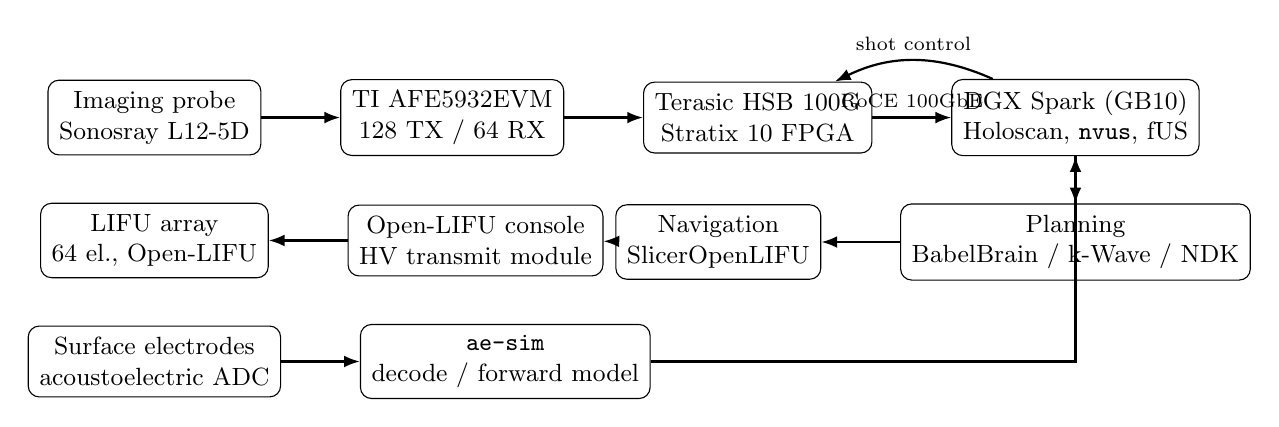
\begin{tikzpicture}[node distance=6mm and 10mm,
  box/.style={draw,rounded corners,align=center,minimum height=9mm,inner sep=4pt,font=\small},
  arr/.style={-{Latex[length=2mm]},thick}]
\node[box] (probe) {Imaging probe\\Sonosray L12-5D};
\node[box,right=of probe] (afe) {TI AFE5932EVM\\128 TX / 64 RX};
\node[box,right=of afe] (hsb) {Terasic HSB 100G\\Stratix 10 FPGA};
\node[box,right=of hsb] (spark) {DGX Spark (GB10)\\Holoscan, \texttt{nvus}, fUS};
\node[box,below=of probe] (lifu) {LIFU array\\64 el., Open-LIFU};
\node[box,right=of lifu] (tx) {Open-LIFU console\\HV transmit module};
\node[box,below=of spark] (plan) {Planning\\BabelBrain / k-Wave / NDK};
\node[box,left=of plan] (nav) {Navigation\\SlicerOpenLIFU};
\node[box,below=of lifu] (ae) {Surface electrodes\\acoustoelectric ADC};
\node[box,right=of ae] (aesim) {\texttt{ae-sim}\\decode / forward model};
\draw[arr] (probe)--(afe); \draw[arr] (afe)--(hsb); \draw[arr] (hsb)--node[above,font=\scriptsize]{RoCE 100GbE}(spark);
\draw[arr] (spark) to[bend right=25] node[above,font=\scriptsize]{shot control}(hsb);
\draw[arr] (tx)--(lifu); \draw[arr] (spark)--(plan); \draw[arr] (plan)--(nav); \draw[arr] (nav)--(tx);
\draw[arr] (ae)--(aesim); \draw[arr] (aesim)-|(spark);
\end{tikzpicture}
\caption{Bench architecture. Solid pieces are published designs; the acoustoelectric row and the loop back from readout to stimulation are the parts we build.}
\end{figure}

\section{Software to build on}\label{sec:software}

All repositories below were checked on 2026-10-25; star counts are indicative only. Forks under \texttt{github.com/m9h} were made the same day.

\begin{longtable}{@{}>{\raggedright\arraybackslash}p{3.3cm}>{\raggedright\arraybackslash}p{2.6cm}>{\raggedright\arraybackslash}p{2.0cm}>{\raggedright\arraybackslash}p{7.2cm}@{}}
\toprule
Project & Origin & Licence & Role for us \\
\midrule
\endhead
\texttt{holoscan-ultrasound-imaging} & NVIDIA & Apache-2.0 (FPGA IP: Altera) & Imaging acquisition, GPU beamforming, per-shot control; the fUS engine. v0.1. \\
\texttt{openlifu-python}, \texttt{openlifu-sdk}, \texttt{openlifu-desktop-application}, \texttt{SlicerOpenLIFU}, \texttt{openlifu-transmitter-fw}, \texttt{openlifu-console-fw}, \texttt{openlifu-verification-tank}, \texttt{OpenLIFU-3DScanner}, \texttt{openlifu-closed-loop-eeg} & Openwater & Apache-2.0 (3DRegistration AGPL) & Stimulation planning, hardware I/O, firmware, planning GUI, neuronavigation, tank control, EEG-triggered sonication. We already fork \texttt{openlifu-python} and ran the Slicer extension on aarch64. \\
\texttt{openlifu-electrical}, \texttt{openlifu-mechanical}, \texttt{openmotion-electrical}, \texttt{openmotion-mechanical} & Openwater & CERN-OHL-S-2.0 & Array flex, HV TX module, console PCB, housings, tank fixtures; Open-Motion PCBs and enclosures. \\
\texttt{openwater-neuromod-hardware}, \texttt{-software}, \texttt{opw\_ustx} & Openwater & AGPL-3.0 & Previous-generation wearable steerable LIFU headset and USTX modules with acoustic validation data \cite{bawiec2025}. \\
\texttt{openmotion-sdk}, \texttt{openmotion-bloodflow-app}, \texttt{openmotion-*-fpga}, \texttt{openmotion-sensor-fw} & Openwater & Apache-2.0 / AGPL-3.0 & Near-infrared optical blood-flow readout; a second haemodynamic channel during sonication. \\
\texttt{openwater-phantoms}, \texttt{openwater-reference-meshes}, \texttt{openlifu-sample-database}, \texttt{openwater-regulatory}, \texttt{openwater-patents} & Openwater & AGPL-3.0 / CC~BY~4.0 & Gelatin/agarose and acousto-optic phantom recipes, rat and vessel moulds, optical headset phantom CAD; one textured head mesh (skull/brain folders empty); transducer and protocol definitions; FDA correspondence; patent list and pledge. \\
\texttt{alephneuro/microbubbles} (Ultratrace ULM) & Aleph Neuro & MIT & GPU (MACH, CUDA 12/13) beamforming from demodulated IQ, temporal SVD clutter filter, 3D bubble localisation, Kalman tracking, 3D viewers; 96\,GB public transcranial dataset. The beamform and SVD stages are most of a fUS pipeline. \\
Neurotech Development Kit (\texttt{neurotechdevkit}) & AE Studio & Apache-2.0 & Teaching-grade TUS simulation and visualisation in Python; the right first week for students. Built by the team that supported Forest. \\
BabelBrain / BabelViscoFDTD & Pichardo lab, Calgary & BSD-3 / \todo{check: NOASSERTION on GitHub} & Prospective TUS planning from CT/MR with GPU FDTD (CUDA, Metal, OpenCL). \texttt{ae-sim} already uses BabelViscoFDTD; we package it for Fedora. \\
k-Wave, j-Wave & UCL (Treeby, Cox, Stanziola) & LGPL-3.0 & Reference acoustic solvers; j-Wave is JAX and differentiable, so it runs on the Spark GPU and can do inverse design of phase maps. \\
Stride & Imperial (Cueto, Guasch) & AGPL-3.0 & Full-waveform inversion and modelling; for skull property estimation. \\
PRESTUS & Donders & GPL-3.0 & End-to-end TUS preprocessing and simulation pipeline (MATLAB/k-Wave) used in human studies; good protocol reference. \\
SimNIBS & DTU/DRCMR & GPL-3.0 & Head models (\texttt{charm}) and lead fields; we build it for Fedora/Debian aarch64, and \texttt{ae-sim} consumes its lead fields. \\
mSOUND & Jing lab & GPL-3.0 & Frequency-domain alternative for fast focus estimates. \\
\texttt{ae-sim} (ours, private) & Morgan Hough / hades-canyon & TBD & Acoustoelectric forward model: BabelViscoFDTD acoustics $\times$ SimNIBS lead fields, scikit-fem, cupy on the Spark. Becomes the decoder design tool. \\
Acoustoelectric (GitHub org) & \todo{check: likely Rintoul} & \todo{check} & Fourier/k-space Poisson and FEM solutions, neural-recording analysis for acoustoelectric data. \\
Open-H-RF v1.0 \cite{openhrf} & Stanford, TU/e, NVIDIA and 38 contributing institutions & CC BY 4.0 & 39\,TB of pre-beamformed channel data in 19,471 zea-format HDF5 files across 33 subsets, hosted as \texttt{nvidia/Open-H-RF} on Hugging Face with a per-subset reconstruction script. The fUS-relevant subsets are \texttt{ulmshare} (99 transcranial mouse-brain ULM acquisitions, $\sim$180\,GB each, to be streamed), \texttt{twente-vortexflow} (flow phantom with simultaneous optical ground truth, 6 files of 1.5\,GB, our first replay target), \texttt{resolvestroke}, \texttt{stanford-murine} and the Waterloo vector-Doppler sets. \\
\texttt{mach} (\texttt{mach-beamform}) \cite{mach} & Forest Neurotech & BSD-3-Clause-Clear & CUDA delay-and-sum written for fUSI, about ten times faster than the prior state of the art, with CuPy/JAX zero-copy bindings; the kernel Aleph's pipeline calls. Wheels are x86\_64 only, so on the Spark it is built from source for sm\_121. \\
\texttt{zea} \cite{zea} & TU/e & Apache-2.0 & Keras-3 ultrasound pipeline (demodulation, beamforming, envelope, log compression) and the loader for the Open-H-RF file format; runs on CPU or GPU. \\
\texttt{nvus-fus} & ours & Apache-2.0 & Phase-0 code: ITRUSST safety supervisor, SVD clutter filter and power-Doppler reference, zea replayer, flow-phantom script; 33 unit tests. \\
3D Slicer + IDC & Kitware / NCI & BSD / CC~BY & Visualisation, registration, CT/MR head data (CC~BY only) for skull models. \\
\bottomrule
\end{longtable}

What \emph{does not} exist as open code, as far as checked: a GPU fUS power-Doppler pipeline on the Holoscan operators (Iconeus's is closed; academic MATLAB code exists; Aleph's MIT pipeline supplies GPU beamforming and SVD clutter filtering offline from IQ files, but not power-Doppler integration or a streaming Holoscan wrapper); a safety supervisor computing $I_{\mathrm{SPPA}}$, $I_{\mathrm{SPTA}}$, MI and thermal index from the live drive settings and refusing out-of-range sonications; a driver that puts Open-LIFU's transmit module under Holoscan shot-level control; and any acoustoelectric decoding software beyond research scripts.

\section{Bill of materials}\label{sec:bom}

Prices are order-of-magnitude estimates (\est) from memory and general vendor knowledge; none has been quoted. Treat the list as a shopping checklist, not a budget. The Holoscan repository is said to contain a component shopping list that should be used as the authoritative source for Part~A \cite{holoscan}.

\subsection*{A. Imaging bench (Holoscan reference design)}
\begin{itemize}[leftmargin=*,nosep]
\item DGX Spark (GB10): \textbf{have}. Its built-in ConnectX-7 ports give the 100/200\,GbE RoCE path \todo{check that the reference design is qualified on the Spark's NIC}.
\item Terasic Holoscan Sensor Bridge 100G (Stratix~10~TX): \$5--8k\est.
\item TI AFE5932EVM evaluation module (AFE5932 $\times$2, TX73L64 $\times$2): \$2--4k\est; plus the TI controller/power boards the EVM needs \todo{check}.
\item Sonosray L12-5\,D linear probe with matching connector: \$1--3k\est.
\item 100\,GbE QSFP28 DAC cable, bench PSU, cabling, enclosure: \$0.5k\est.
\item Imaging phantoms: a CIRS or home-made agar/graphite flow phantom with a pump for Doppler: \$0.3--3k\est.
\end{itemize}
Subtotal roughly \$10--18k\est, consistent with the \$10k figure in the announcement \cite{simson2026}.

\subsection*{B. Stimulation bench (Open-LIFU)}
\begin{itemize}[leftmargin=*,nosep]
\item Either a complete Open-LIFU console and 64-element transducer from Openwater (price on request; OEM configurations exist \cite{openlifu}), or fabricate from \texttt{openlifu-electrical}: array flex, transmit module Rev~0.4.1, console PCB, HV supply, housings from \texttt{openlifu-mechanical}. PCB fabrication and assembly \$3--8k\est; piezo elements and lens/matching are the hard part and may need a vendor.
\item Alternative single-element start: a Sonic Concepts H-series 250--500\,kHz focused transducer with matching network (\$8--15k\est) and an RF amplifier (E\&I 1040L or similar, \$8--12k\est) driven by an arbitrary waveform generator (\$1--2k\est). Slower to steer but calibratable on day one.
\end{itemize}

\subsection*{C. Characterisation and safety (not optional)}
\begin{itemize}[leftmargin=*,nosep]
\item Needle or fibre-optic hydrophone with preamp (Onda HNR-series or Precision Acoustics): \$5--15k\est.
\item Water tank with 3-axis positioner (Open-LIFU verification tank design, or a 3D-printer gantry) and degasser: \$2--6k\est.
\item Radiation force balance for total power: \$3--6k\est, or a home-built one.
\item Skull-mimicking phantoms (3D-printed from CT, or ex-vivo skull caps under institutional rules): \$0.5--2k\est.
\item Oscilloscope $\geq$\,200\,MHz, current probe: \$2--4k\est.
\end{itemize}

\subsection*{D. Navigation and acoustoelectric}
\begin{itemize}[leftmargin=*,nosep]
\item Optical tracking: NDI Polaris Vega (\$15--25k\est) or, to start, two webcams and ArUco markers with the Open-LIFU 3D-scanner workflow (\$0.2k\est).
\item Acoustoelectric readout: low-noise multichannel amplifier with bandwidth above the ultrasound frequency (an OpenBCI board is far too slow); options are an Intan/RHD-class front end with external high-rate ADC, a Red Pitaya or Digilent ADC board, or the imaging AFE itself in receive-only mode: \$0.5--3k\est. Saline tank with electrodes and a signal source for heterodyning experiments: \$0.3k\est.
\end{itemize}

\subsection*{E. Compute}
The DGX Spark covers acquisition, simulation (BabelViscoFDTD with cupy; j-Wave with JAX) and planning. Memory is the shared 120\,GB pool; caps must be set on every CUDA process (we have hit box-wide OOM freezes on it). Fedora/Debian aarch64 packaging of SimNIBS, BabelViscoFDTD, FreeSurfer and 3D~Slicer is already our work in neurofedora/neurodebian.

\section{What we would have to build}

\begin{enumerate}[leftmargin=*]
\item \textbf{fUS pipeline on Holoscan.} Operators for 32-angle compounding, SVD clutter rejection, power Doppler, and a live CBV map; start from Aleph's \texttt{microbubbles} beamform and SVD stages (MIT) and wrap them as streaming Holoscan operators; validate against a flow phantom, Aleph's public dataset, and Open-H-RF or published rat fUS data. Deliverable: \texttt{nvus-fus} Python package. This alone is a publishable student project.
\item \textbf{Safety supervisor.} A small service that takes transducer calibration (from Part~C), drive settings and the plan, computes the transcranial mechanical index, predicted temperature rise and peak temperature, cranial thermal index against the ITRUSST exposure-time table, and thermal dose (CEM43) against the ITRUSST consensus levels \cite{itrusst}, reports the FDA Track-3 derated $I_{\mathrm{SPPA}}$/$I_{\mathrm{SPTA}}$ for reference, logs every sonication, and gates the HV enable. A first version with unit tests exists in \texttt{nvus-fus}; it is to be reviewed by the advisor before any transducer is energised.
\item \textbf{Stimulation driver integration.} Bring Open-LIFU's console under the same host and clock as the imaging chain, through \texttt{openlifu-sdk}, so that a sonication can be triggered between imaging frames and the fUS response captured. Interleaving at the shot level is what the Holoscan design is built for. Open-Motion's optical readout can be added as a third, independent channel through \texttt{openmotion-sdk}.
\item \textbf{Planning glue.} A reproducible path from CT/MR (IDC CC~BY data, or phantoms) through SimNIBS \texttt{charm} and BabelBrain to element phases for the Open-LIFU array, with j-Wave for optimisation. We have most of this packaged already.
\item \textbf{Acoustoelectric path.} Use \texttt{ae-sim} to design electrode layouts and ultrasound focus parameters for a saline/gel phantom with an injected current, then build the heterodyne receiver and reproduce Rintoul 2023 on the bench. This is where Jean Rintoul's advice has the most leverage and where the result is new.
\item \textbf{Mechanical.} Probe and array holders, a head phantom fixture, and a shared coordinate frame with fiducials; all 3D-printed, designs in the repo.
\item \textbf{Packaging and reproducibility.} Containers (aarch64 first) for every software piece, continuous phantom tests, and documented calibration files, so another group can rebuild the bench from the repository.
\end{enumerate}

\section{Plan}

\paragraph{Phase 0, software only (weeks 1--6).} Install NDK, j-Wave, BabelBrain and \texttt{openlifu-python} on the Spark; reproduce a transcranial focus through a CT-derived skull with each; run \texttt{ae-sim} end to end; replay Open-H-RF data through a beamform, SVD and power-Doppler chain; build \texttt{mach} for the Spark and run Aleph's pipeline on its sample; write the safety supervisor as pure software with unit tests. Output: a reproduced-simulation report and the supervisor. Status at this draft: the replay chain runs on the Twente flow phantom (CPU; GPU pending JAX CUDA~13 on aarch64), the supervisor v0 passes its tests, \texttt{mach} is being built for sm\_121, and the Aleph sample is downloading.

\paragraph{Phase 1, imaging bench (weeks 6--16).} Purchase Part~A; bring up the Holoscan design; B-mode, then plane-wave compounding, then Doppler on a flow phantom; fUS pipeline on the GPU. Output: live power-Doppler of a phantom at $\geq$\,10\,fps.

\paragraph{Phase 2, stimulation bench (weeks 12--24).} Purchase Part~C first, then Part~B. Hydrophone-map the transducer, fit the calibration, run the planning chain to a target in a skull phantom and verify focus position and pressure against the plan. Output: a calibrated, navigated, phantom-verified LIFU focus with logged exposure metrics.

\paragraph{Phase 3, acoustoelectric (weeks 16--30).} Saline tank, injected current, heterodyne readout at the ultrasound frequency; compare with \texttt{ae-sim} predictions; move to a conductive head phantom. Output: reproduction of focused acoustoelectric decoding with open hardware.

\paragraph{Phase 4, integration (weeks 24--36).} Interleaved stimulate-then-image on a phantom with a thermal or flow response; one shared coordinate frame; a closed-loop demo (stimulation parameter updated from the imaging readout). Output: the bench described in this document, and a paper.

\paragraph{Governance.} Phantom and bench only. No human or animal use is proposed; any such step requires institutional review, the ITRUSST limits as a floor, and the advisor's sign-off on the safety supervisor. Hardware files stay under CERN-OHL-S where derived from Open-LIFU; our software under Apache-2.0; the Altera FPGA IP terms are respected by keeping it out of our repository and pointing to NVIDIA's.

\section{Open questions and risks}
\begin{itemize}[leftmargin=*,nosep]
\item Is the Holoscan container qualified on the DGX Spark, or only on the host its README calls PGX? The project page and README disagree \cite{holoscan}. Ask before purchase.
\item Terasic HSB 100G lead time and whether a 100\,GbE port on the Spark can be dedicated to it while the box stays on the lab network.
\item Open-LIFU's transducer: can students fabricate the array, or must it be bought? Openwater's price is unknown.
\item The imaging probe (5--12\,MHz) cannot do transcranial human fUS; rodent-scale and through-window imaging only, which matches Arbor's own first device. A 2--8\,MHz probe or a matrix array for volumetric fUS would be a later purchase.
\item Memory safety on the shared Spark: every CUDA process capped; the box has frozen under unbounded allocations before.
\item Export and licence hygiene: no MimickNet weights (CC~BY-NC) in anything shared; IDC data filtered to CC~BY; Openwater derivatives keep their per-repository licence (Apache, AGPL or CERN-OHL-S).
\item Patents (Section~\ref{sec:ip}): phantom work is safe; any later human protocol must be checked against the Stanford TBS-LIFU claims and the Forest imaging-plus-modulation family; NVIDIA, Butterfly and Nudge filings may still be unpublished.
\item The Nolan Williams filing is Stanford's; its prosecution and licensing now rest with Stanford OTL, not the lab.
\end{itemize}

\begin{thebibliography}{99}\small
\bibitem{martin2025} E.~Martin, M.~Roberts, I.~F.~Grigoras, O.~Wright, T.~Nandi, S.~W.~Rieger, J.~Campbell, T.~den~Boer, B.~T.~Cox, C.~J.~Stagg, B.~E.~Treeby. Ultrasound system for precise neuromodulation of human deep brain circuits. \emph{Nature Communications} 16 (2025). doi:10.1038/s41467-025-63020-1. UCL/Oxford press releases, 9 Sept 2025.
\bibitem{simson2026} W.~Simson. ``We made an open-source ultrasound machine.'' LinkedIn post, Oct 2026 (\url{https://lnkd.in/p/grq4nQcY}).
\bibitem{holoscan} NVIDIA Holoscan Ultrasound Imaging Reference Design. \url{https://www.holoscan.org/reference-designs/ultrasound/}; \url{https://github.com/nvidia-holoscan/holoscan-ultrasound-imaging} (v0.1, Apache-2.0; FPGA IP under Altera licence). Read 2026-10-25.
\bibitem{openlifu} Openwater. Open-LIFU. \url{https://www.openwater.health/openlifu}; Kitware, ``OpenLIFU: accelerating focused ultrasound research with open source hardware and 3D Slicer driven software''; Clinical Research News, 25 July 2025 (MIT Lincoln Laboratory deployment); 27 Jan 2026 (investigational status).
\bibitem{openlifu_hw} \url{https://github.com/OpenwaterHealth/openlifu-electrical} (CERN-OHL-S-2.0; 64-element array flex, transmit module Rev~0.4.1, console PCB); \url{https://github.com/OpenwaterHealth/openlifu-mechanical}; \url{https://github.com/OpenwaterHealth/openlifu-python} (Apache-2.0); \url{https://github.com/OpenwaterHealth/SlicerOpenLIFU} (Apache-2.0).
\bibitem{nudge} Contrary Research, ``Nudge''; Newswise / FUS Foundation, ``Study explores neuromodulation for essential tremor symptoms''; Techleap, ``Nudge Zero enters human trials following \$100M raise''; Thrive Capital job postings (Mar 2026).
\bibitem{forest1} UK HRA research summary ``Forest 1''; BHR Hospitals NHS Trust, ``\pounds6.5m award: brain changer''; University of Plymouth, ``\pounds6.5m project aims to revolutionise mental health treatment using ultrasound''; Digital Health, 2025.
\bibitem{arbor} Arbor Neuroscience job postings via xtalks.com (``Arbor is a Focused Research Organization within the Convergent Research family, and the new name for Forest Neurotech''; ``Forest 1 ultrasound system \ldots{} will soon stimulate as well'').
\bibitem{merge} \emph{Wired}, Dec 2025 (Merge Labs spun out of Forest Neurotech); BioPharmaTrend / Parsers.vc, Jan 2026 (\$252M seed, OpenAI, Bain Capital, Gabe Newell).
\bibitem{aestudio} AE Studio, ``Neurotechnology consulting'' and Medical Design \& Outsourcing, ``Software developed for brain-computer interfaces'' (AE supports Forest Neurotech's data science and software); \url{https://github.com/agencyenterprise/neurotechdevkit} (Apache-2.0).
\bibitem{iconeus_story} Iconeus, ``Our story'' (\url{https://iconeus.com/our-story/}); Physics for Medicine Paris, ``Creation of Iconeus startup company to widely spread fUS imaging modality.''
\bibitem{iconeus_one} Iconeus One product page (\url{https://iconeus.com/iconeus-one/}).
\bibitem{iconeus_us} Iconeus Inc.\ press release, March 2026.
\bibitem{rintoul} J.~Rintoul et al. Remote focused encoding and decoding of electric fields through acoustoelectric heterodyning. \emph{Communications Physics} (2023); J.~Rintoul, review of simple ultrasound hardware, \emph{Journal of Open Hardware} (2022); Imperial College DRI alumni page; Foresight Institute talk ``Toward scalable non-invasive neurotech using the acoustoelectric effect'' (2026). \todo{add DOIs}
\bibitem{openwater_gh} \url{https://github.com/OpenwaterHealth} (56 repositories, licences and push dates read via the GitHub API on 2026-10-25); \url{https://github.com/OpenwaterHealth/openlifu-sdk}; \url{https://github.com/OpenwaterHealth/openwater-neuromod-hardware}.
\bibitem{openwater_docs} Openwater Documentation, \url{https://docs.openwater.health/} (Open-LIFU and Open-Motion; ``AGPL 3.0'' software, ``CC BY-SA 4.0'' hardware; investigational, research use only). Read 2026-10-25.
\bibitem{openwater_open} Openwater blog, ``Inside Open-LIFU: how we open-sourced a focused-ultrasound research platform'' and ``Building the community: how open source is reshaping medical device development''; The Sociable, Jan 2024 (open-sourcing announcement).
\bibitem{bawiec2025} C.~Bawiec et al. A wearable, steerable, transcranial low-intensity focused ultrasound system. \emph{Journal of Ultrasound in Medicine} 44 (2025). doi:10.1002/jum.16600; PMC11719763; medRxiv 2023.12.22.23300243.
\bibitem{openwater_patents} \url{https://github.com/OpenwaterHealth/openwater-patents}: portfolio list (68 filings) and Patent Pledge (open-source medical devices on CC~BY-SA designs or AGPL-type code; defensive termination). Read 2026-10-25.
\bibitem{bfly_forest} Butterfly Network press release, 24 Oct 2023: five-year co-development agreement with Forest Neurotech for ultrasound-on-chip brain--computer interfaces.
\bibitem{bfly_aleph} Butterfly Network press release, 25 June 2026, ``Butterfly Network's Embedded partner Aleph Neuro unveils stunning brain images''; MassDevice, same day.
\bibitem{aleph} Aleph Neuro (\url{https://alephneuro.com}); Neurofounders, ``Aleph Neuro joins the ultrasound wave in BCI'' (Aug 2026); Noze, ``Aleph Neuro: ultrasound brain imaging, fully open source.''
\bibitem{aleph_repo} \url{https://github.com/alephneuro/microbubbles}, ``Pipeline and dataset for reproducing 3D transcranial ultrasound localization microscopy'' (MIT; 127 stars; last push 2026-07-31). Read 2026-10-25.
\bibitem{bfly_merge} Butterfly Network press release, 1 Sept 2026, ``Merge Labs and Butterfly Network partner to advance ultrasound-based brain-computer interfaces'' (Poseidon family; exclusive BCI R\&D platform; BCI Innovation Summit 2 Sept 2026); MobiHealthNews.
\bibitem{bfly_bridge} Butterfly Network press release, 6 Oct 2026, ``Bridge Neurotech and Butterfly Network announce partnership to develop fully non-invasive brain-computer interface''; MassDevice, 7 Oct 2026 (\$13.5M; Biederman).
\bibitem{bfly_midjourney} Butterfly Network press release, 18 June 2026, ``Butterfly Network provides commentary on Midjourney Medical's full body ultrasound scanner announcement'' (40 modules per system; up to \$74M over five years; 8-K of 17 Nov 2025); Midjourney blog ``A new era of Midjourney'', 17 June 2026; Radiology Business; The Next Web; Engadget.
\bibitem{gestala} Neurofounders, ``Gestala raises RMB 420M to scale its ultrasound BCI thesis'' (July 2026).
\bibitem{forest_patent} US\,2025/0001217\,A1, Forest Neurotech LLC, ``Systems and methods for imaging and modulating the nervous system using an ultrasound-based brain-computer interface''. \url{https://patents.google.com/patent/US20250001217A1}. Read 2026-10-25.
\bibitem{williams_patent} N.~R.~Williams, J.~Coetzee. ``Systems and methods for transcranial focused ultrasound neurostimulation.'' WO\,2024/030928\,A2 (8 Feb 2024); US\,2026/0041941\,A1 (12 Feb 2026), application 19/100,561; assignee Leland Stanford Junior University; priority 1 Aug 2022. \url{https://patents.google.com/patent/US20260041941A1/en}. Read 2026-10-25. Stanford Medicine obituary, Dec 2025.
\bibitem{attune} Justia, patents assigned to Attune Neurosciences, Inc.\ (US\,11,730,960; US\,12,485,297 / US\,2025/0108235\,A1); PitchBook and Crunchbase profiles (2026); Neurofounders profile.
\bibitem{bfly_ip} Butterfly Network, ``Ultrasound-on-Chip technology'' (\url{https://www.butterflynetwork.com/technology}; ``over 600 patents''); Radiology Business and MassDevice on Fujifilm Sonosite v.\ Butterfly Network (2023, seven patents); Justia assignee listing.
\bibitem{insightec} AuntMinnie, FDA clearance of Exablate for staged bilateral Parkinson's treatment (July 2025); FUS Foundation, ``Insightec announces new company, Lotus Neuro'' (Dec 2025).
\bibitem{fusf_ip} Focused Ultrasound Foundation, ``Intellectual property'' page (US\,12,599,785\,B2, Fondazione IRCCS Besta / INRiM, 14 Apr 2026) and ``State of the Field 2023, Chapter 8: FUS industry''; \emph{Brain Stimulation} 2026, registry-based analysis of global TUS trials (device counts).
\bibitem{patsnap} PatSnap, ``Transcranial focused ultrasound neuromodulation 2026'' and ``Non-invasive deep brain neuromodulation patents: top companies and trends 2026'' (secondary; indicative only).
\bibitem{kwave} B.~E.~Treeby, B.~T.~Cox. k-Wave. \url{https://github.com/ucl-bug/k-wave} (LGPL-3.0).
\bibitem{jwave} A.~Stanziola et al. j-Wave. \url{https://github.com/ucl-bug/jwave} (LGPL-3.0).
\bibitem{itrusst} J.-F. Aubry, D. Attali, M. E. Schafer, E. Fouragnan, C. F. Caskey, R. Chen, G. Darmani, E. J. Bubrick, J. Sallet, C. R. Butler, C. J. Stagg, M. C. Klein-Fl\"ugge, S.-S. Yoo, C. K. Holland, B. Treeby, E. Martin, L. Verhagen, K. Butts Pauly. ITRUSST consensus on biophysical safety for transcranial ultrasound stimulation. \emph{Brain Stimulation} 18(6):1896--1905, 2025. doi:10.1016/j.brs.2025.10.007 (arXiv:2311.05359).
\bibitem{openhrf} T. S. W. Stevens, S. W. Penninga, W. L. van Nierop, O. Nolan, \emph{et al.}, J. J. Dahl, R. J. G. van Sloun, W. Simson. OpenH-RF: a large-scale ultrasound raw channel dataset initiative. arXiv:2610.13616, 9 October 2026. Data: \url{https://huggingface.co/datasets/nvidia/Open-H-RF} (CC BY 4.0); code: \url{https://github.com/open-h/Open-H-RF}.
\bibitem{mach} C. Guan, A. P. Rockhill, M. Sode, G. Pinton. mach: ultrafast ultrasound beamforming. \emph{Journal of Medical Imaging} 13(6):062203, 2026. doi:10.1117/1.JMI.13.6.062203. \url{https://github.com/Forest-Neurotech/mach} (BSD-3-Clause-Clear).
\bibitem{zea} TU/e Biomedical Diagnostics Lab. zea: a toolbox for cognitive ultrasound imaging. \url{https://github.com/tue-bmd/zea}, v0.1.8, 2026 (Apache-2.0).
\end{thebibliography}

\end{document}
